$  $\chapter{Arhitektura i dizajn sustava}
		
		\textbf{\textit{dio 1. revizije}}\\

		\textit{ Potrebno je opisati stil arhitekture te identificirati: podsustave, preslikavanje na radnu platformu, spremišta podataka, mrežne protokole, globalni upravljački tok i sklopovsko-programske zahtjeve. Po točkama razraditi i popratiti odgovarajućim skicama:}
	\begin{itemize}
		\item 	\textit{izbor arhitekture temeljem principa oblikovanja pokazanih na predavanjima (objasniti zašto ste baš odabrali takvu arhitekturu)}
		\item 	\textit{organizaciju sustava s najviše razine apstrakcije (npr. klijent-poslužitelj, baza podataka, datotečni sustav, grafičko sučelje)}
		\item 	\textit{organizaciju aplikacije (npr. slojevi frontend i backend, MVC arhitektura) }		
	\end{itemize}

	
		

		

				
		\section{Baza podataka}
			
			\textbf{\textit{dio 1. revizije}}\\
			
		\textit Za naš projekt odabrali smo relacijsku bazu podataka zbog njezine pogodnosti da prikaže mali dio stvarnog svijeta bez redundancije unutar same baze. dohvaćanje podataka je jako brzo i jako lagano se može paralelizirati. \\
Naša baza podataka sastoji se od sljedećih tablica:
\begin{itemize}

\item
	user
\item
	friends
\item
	friendship-req
\item
	role
\item
	event
\item
	event-attendance
\item
	event-path
\item
	path
\item
	badge
\item
	user-badge
\item
	notification
\item
	hill
\item
	mountain-lodge
\item
	utility
\item
	lodge-utility
\item
	path-user-grade
\item
	path-wishlist
\item
	completed-paths
\item
	report-path
\item
	visit-confirmation-request
\item
	mountaneer-on-duty
	


\end{itemize}
		
			\subsection{Opis tablica}
			
%Tablice
			\textit{\textbf{user}  Ovaj entitet sadrži sve važne informacije o korisniku aplikacije. Sadrži atribute: name, email, password, image, role-id.  Ova tablica je u Many-to-One vezi s tablicom role preko atributa korisnika role-id.}
			
			\begin{longtabu} to \textwidth {|X[6, l]|X[6, l]|X[20, l]|}
				
				\hline \multicolumn{3}{|c|}{\textbf{user - ime tablice}}	 \\[3pt] \hline
				\endfirsthead
				
				\hline \multicolumn{3}{|c|}{\textbf{user - ime tablice}}	 \\[3pt] \hline
				\endhead
				
				\hline 
				\endlastfoot
				
				\cellcolor{LightGreen}id & INT	&  	jedinstveni identifikator korisnika	\\ \hline
				name	& VARCHAR &  ime i prezime korisnika 	\\ \hline 
				email & VARCHAR &  email korisnika \\ \hline 
				password & VARCHAR	&  	lozinka korisnika	\\ \hline 
				image & byea	&  	slika korisnika	\\ \hline 
				role-id & FOREIGN-KEY(role-id)	&  	strani ključ uloge korisnika	\\ \hline 
				%\cellcolor{LightBlue} primjer	& VARCHAR &   	\\ \hline 
				
				
			\end{longtabu}
		
			\textit{\textbf{friends} Ovaj entitet sadrži informaciju o Many-To-Many prijateljskoj vezi između dva korisnika. Sadrži atribute: user-1, user-2, koji su oba strani ključevi iz tablice user}
			
			\begin{longtabu} to \textwidth {|X[6, l]|X[6, l]|X[20, l]|}
				
				\hline \multicolumn{3}{|c|}{\textbf{friends - ime tablice}}	 \\[3pt] \hline
				\endfirsthead
				
				\hline \multicolumn{3}{|c|}{\textbf{friends - ime tablice}}	 \\[3pt] \hline
				\endhead
				
				\hline 
				\endlastfoot
				
				\cellcolor{LightGreen}user-1 & FOREIGN-KEY(user)	&  strani ključ 1. korisnika	\\ \hline
				user-2	& FOREIGN-KEY(user) &   strani ključ 2. korisnika	\\ \hline 
				%\cellcolor{LightBlue} primjer	& VARCHAR &   	\\ \hline 
				
				
			\end{longtabu}

			\textit{\textbf{friendship-req} Ovaj entitet sadrži informaciju o Many-To-Many poslanom zahtjevu za prijateljstvo između 2 korisnika. Sadrži atribute: friendship-send, friendship-recieve, koji su oba strani ključevi iz tablice user}
			
			\begin{longtabu} to \textwidth {|X[6, l]|X[6, l]|X[20, l]|}
				
					\hline \multicolumn{3}{|c|}{\textbf{friendship-req - ime tablice}}	 \\[3pt] \hline
				\endfirsthead
				
				\hline \multicolumn{3}{|c|}{\textbf{friendship-req - ime tablice}}	 \\[3pt] \hline
				\endhead
				
				\hline 
				\endlastfoot
				
				\cellcolor{LightGreen}friendship-send & FOREIGN-KEY(user)	&  strani ključ korisnika koji šalje zahtjev za prijateljstvom 	\\ \hline
				friendship-recieve	& FOREIGN-KEY(user) &   strani ključ korisnika koji prima zahtjev za prijateljstvom	\\ \hline 
				%\cellcolor{LightBlue} primjer	& VARCHAR &   	\\ \hline 
				
				
			\end{longtabu}
		
			\textit{\textbf{role} Ovaj entitet sadrži informaciju o ulozi koju ima određeni korisnik. Određuje razinu dozvole korisnika}
			
			\begin{longtabu} to \textwidth {|X[6, l]|X[6, l]|X[20, l]|}
				
				\hline \multicolumn{3}{|c|}{\textbf{role - ime tablice}}	 \\[3pt] \hline
				\endfirsthead
				
				\hline \multicolumn{3}{|c|}{\textbf{role - ime tablice}}	 \\[3pt] \hline
				\endhead
				
				\hline 
				\endlastfoot
				
				\cellcolor{LightGreen}id & int	&  jedinstveni ID uloge	\\ \hline
				name	& VARCHAR &  ime uloge 	\\ \hline 
				%\cellcolor{LightBlue} primjer	& VARCHAR &   	\\ \hline 

			\end{longtabu}

			\textit{\textbf{event} Ovaj entitet sadrži informaciju o događaju. Sadrži atribute: name, description, start-date, end-date, date-created i u One-To-Many je vezi s tablicom user preko atributa author-id.}
			
			\begin{longtabu} to \textwidth {|X[6, l]|X[6, l]|X[20, l]|}
				
				\hline \multicolumn{3}{|c|}{\textbf{event - ime tablice}}	 \\[3pt] \hline
				\endfirsthead
				
				\hline \multicolumn{3}{|c|}{\textbf{event - ime tablice}}	 \\[3pt] \hline
				\endhead
				
				\hline 
				\endlastfoot
				
				\cellcolor{LightGreen}id & int	&  	jedinstveni id događaja 	\\ \hline
				name	& VARCHAR & ime događaja  	\\ \hline 
				description & VARCHAR &  opis događaja \\ \hline 
				start-date & timestamp	&  	datum početka događaja	\\ \hline 
				end-date & timestamp	&  	datum kraja događaja	\\ \hline 
				date-created & timestamp	&  	datum stvaranja događaja	\\ \hline 
				author-id & FOREIGN-KEY(user)	& strani ključ korisnika koji je stvorio događaj 		\\ \hline 
				%\cellcolor{LightBlue} primjer	& VARCHAR &   	\\ \hline 
				
				
			\end{longtabu}


			\textit{\textbf{event-attendance} Ovaj entitet sadrži informaciju o Many-To-Many učestvovanju na nekom događaju nekog korisnika. Sadrži atribute: user-id, event-id koji su oba strani ključevi.}
			
			\begin{longtabu} to \textwidth {|X[6, l]|X[6, l]|X[20, l]|}
				
				\hline \multicolumn{3}{|c|}{\textbf{event-attendance - ime tablice}}	 \\[3pt] \hline
				\endfirsthead
				
				\hline \multicolumn{3}{|c|}{\textbf{event-attendance - ime tablice}}	 \\[3pt] \hline
				\endhead
				
				\hline 
				\endlastfoot
				
				\cellcolor{LightGreen}user-id & FOREIGN-KEY(user)	&  	strani ključ korisnika 	\\ \hline
				event-id	& FOREIGN-KEY(user) &  strani ključ događaja 	\\ \hline 
				%\cellcolor{LightBlue} primjer	& VARCHAR &   	\\ \hline 
				
				
			\end{longtabu}
		
			
			\textit{\textbf{event-path} Ovaj entitet sadrži informaciju o Many-To-Many vezi između staze i nekog događaja. Sadrži atribute: path-id, event-id koji su oba strani ključevi.}
			
			\begin{longtabu} to \textwidth {|X[6, l]|X[6, l]|X[20, l]|}
				
				\hline \multicolumn{3}{|c|}{\textbf{event-path - ime tablice}}	 \\[3pt] \hline
				\endfirsthead
				
				\hline \multicolumn{3}{|c|}{\textbf{event-path - ime tablice}}	 \\[3pt] \hline
				\endhead
				
				\hline 
				\endlastfoot
				
				\cellcolor{LightGreen}path-id & FOREIGN-KEY(path)	&  	strani ključ staze 	\\ \hline
				event-id	& FOREIGN-KEY(user) &  strani ključ događaja 	\\ \hline 
				%\cellcolor{LightBlue} primjer	& VARCHAR &   	\\ \hline 
				
				
			\end{longtabu}


			\textit{\textbf{path} Ovaj entitet sadrži informacije o pojedinoj stazi. Sadrži atribute: name, start, end, avg-walk-time, length, sea-level-diff, date-created, is-private, author-id, hill-id}
			
			\begin{longtabu} to \textwidth {|X[6, l]|X[6, l]|X[20, l]|}
				
				\hline \multicolumn{3}{|c|}{\textbf{path - ime tablice}}	 \\[3pt] \hline
				\endfirsthead
				
				\hline \multicolumn{3}{|c|}{\textbf{path - ime tablice}}	 \\[3pt] \hline
				\endhead
				
				\hline 
				\endlastfoot
				
				\cellcolor{LightGreen}id & int	&  	jedinstveni ID staze	\\ \hline
				name	& VARCHAR &   ime staze	\\ \hline 
				start & VARCHAR & ime početne staze  \\ \hline 
				end & VARCHAR &  ime završne staze \\ \hline 
				avg-walk-time & time &  prosječno vrijeme potrebno za prolazak staze \\ \hline 
				length & int &  dužina staze u km \\ \hline 
				sea-level-dfiff & int & visinska razlika između početka i kraja staze  \\ \hline 
				date-created & date &  datum stvaranja staze \\ \hline 
				is-private & boolean	&  je li staza dostupna javnosti		\\ \hline 
				author-id & FOREIGN-KEY(user)	&  	strani ključ korisnika koji je kreirao stazu	\\ \hline 
				hill-id & FOREIGN-KEY(hill)	&  strani ključ visočja na kojemu se staza nalazi		\\ \hline 
				%\cellcolor{LightBlue} primjer	& VARCHAR &   	\\ \hline 
				
				
			\end{longtabu}

			\textit{\textbf{badge} Ovaj entitet sadrži informaciju o bedževima koje korisnici mogu osvojiti za neka dostignuća. Sadrže atribute id, name i image}

			\begin{longtabu} to \textwidth {|X[6, l]|X[6, l]|X[20, l]|}
				
				\hline \multicolumn{3}{|c|}{\textbf{badge - ime tablice}}	 \\[3pt] \hline
				\endfirsthead
				
				\hline \multicolumn{3}{|c|}{\textbf{badge - ime tablice}}	 \\[3pt] \hline
				\endhead
				
				\hline 
				\endlastfoot
				
				\cellcolor{LightGreen}id	& int &   jedinstveni id bedža	\\ \hline 
				name & VARCHAR &  ime bedža \\ \hline 
				image & bytea	&  	slika bedža	\\ \hline 
				%\cellcolor{LightBlue} primjer	& VARCHAR &   	\\ \hline 
				
				
			\end{longtabu}
		
		
			\textit{\textbf{friendship-req} Ovaj entitet sadrži informaciju o Many-To-Many odnosu između bedževa i korisnika. Sadrži atribute: user-id, badge-id i date-recieved}
		
			\begin{longtabu} to \textwidth {|X[6, l]|X[6, l]|X[20, l]|}
				
				\hline \multicolumn{3}{|c|}{\textbf{user-badge - ime tablice}}	 \\[3pt] \hline
				\endfirsthead
				
				\hline \multicolumn{3}{|c|}{\textbf{user-badge - ime tablice}}	 \\[3pt] \hline
				\endhead
				
				\hline 
				\endlastfoot
				
				\cellcolor{LightGreen}user-id & FOREIGN-KEY(user)	&  strani ključ korisnika kojemu je pripisan pojedini bedž\\ \hline
				badge-id	& FOREIGN-KEY(badge) &  strani ključ bedža kojega je dobio pojedini korisnik 	\\ \hline 
				date-recieved & date & datum dobivanja pojedinog bedža  \\ \hline 
				%\cellcolor{LightBlue} primjer	& VARCHAR &   	\\ \hline 
				
				
			\end{longtabu}
		
			\textit{\textbf{notification} Ovaj entitet sadrži informaciju o Many-To-Many odnosu između bedževa i korisnika, ali samo u smislu notificiranja korisnika. Kada korisnik potvrdi da je primio notifikaciju, pojedini unos se briše iz ovog entiteta . Sadrži atribute: user-id, badge-id}
			
			\begin{longtabu} to \textwidth {|X[6, l]|X[6, l]|X[20, l]|}
				
				\hline \multicolumn{3}{|c|}{\textbf{notification - ime tablice}}	 \\[3pt] \hline
				\endfirsthead
				
				\hline \multicolumn{3}{|c|}{\textbf{notification - ime tablice}}	 \\[3pt] \hline
				\endhead
				
				\hline 
				\endlastfoot
				
				\cellcolor{LightGreen}user-id & FOREIGN-KEY(user)	&  strani ključ korisnika kojemu je pripisan pojedini bedž\\ \hline
				badge-id	& FOREIGN-KEY(badge) &  strani ključ bedža kojega je dobio pojedini korisnik \\ \hline 
				%\cellcolor{LightBlue} primjer	& VARCHAR &   	\\ \hline 
				
				
			\end{longtabu}
		
		
			\textit{\textbf{hill} Ovaj entitet sadrži informaciju o pojedinom visočju. Sadrži atribute: id i name}
			
			\begin{longtabu} to \textwidth {|X[6, l]|X[6, l]|X[20, l]|}
				
				\hline \multicolumn{3}{|c|}{\textbf{hill - ime tablice}}	 \\[3pt] \hline
				\endfirsthead
				
				\hline \multicolumn{3}{|c|}{\textbf{hill - ime tablice}}	 \\[3pt] \hline
				\endhead
				
				\hline 
				\endlastfoot
				
				\cellcolor{LightGreen}id & int	&  jedinstveni ID visočja 	\\ \hline
				name	& VARCHAR &  ime visočja 	\\ \hline 
				%\cellcolor{LightBlue} primjer	& VARCHAR &   	\\ \hline 
				
				
			\end{longtabu}
		
		
			\textit{\textbf{mountain-lodge} Ovaj entitet sadrži informaciju o planinarskom domu. Sadrži atribute: id, name, image i One-To-Many vezu između visočja hill-id.}
			
			\begin{longtabu} to \textwidth {|X[6, l]|X[6, l]|X[20, l]|}
				
				\hline \multicolumn{3}{|c|}{\textbf{mountain-lodge - ime tablice}}	 \\[3pt] \hline
				\endfirsthead
				
				\hline \multicolumn{3}{|c|}{\textbf{mountain-lodge - ime tablice}}	 \\[3pt] \hline
				\endhead
				
				\hline 
				\endlastfoot
				
				\cellcolor{LightGreen}id & int	&  	jedinstveni ID planinarskog doma 	\\ \hline
				name	& VARCHAR &   ime planinarskog doma	\\ \hline 
				image & bytea &  slika planinarskog doma \\ \hline 
				hill-id & FOREIGN-KEY(hill)	&  strani ključ visočja na kojemu je planinarski dom		\\ \hline 
				%\cellcolor{LightBlue} primjer	& VARCHAR &   	\\ \hline 
				
				
			\end{longtabu}
		
		
		
			\textit{\textbf{utility} Ovaj entitet sadrži informaciju o komunalijama}

			\begin{longtabu} to \textwidth {|X[6, l]|X[6, l]|X[20, l]|}
				
				\hline \multicolumn{3}{|c|}{\textbf{utility - ime tablice}}	 \\[3pt] \hline
				\endfirsthead
				
				\hline \multicolumn{3}{|c|}{\textbf{utility - ime tablice}}	 \\[3pt] \hline
				\endhead
				
				\hline 
				\endlastfoot
				
				\cellcolor{LightGreen}id & int	&  jedinstveni ID komunalije\\ \hline
				name	& VARCHAR &  ime komunalije \\ \hline 
				%\cellcolor{LightBlue} primjer	& VARCHAR &   	\\ \hline 
				
			\end{longtabu}
		
		
			\textit{\textbf{lodge-utility} Ovaj entitet sadrži informaciju o Many-To-Many odnosu između komunalija i planinarskih domova. Sadrži atribute: lodge-id, utility-id}
			
			\begin{longtabu} to \textwidth {|X[6, l]|X[6, l]|X[20, l]|}
				
				\hline \multicolumn{3}{|c|}{\textbf{lodge-utility - ime tablice}}	 \\[3pt] \hline
				\endfirsthead
				
				\hline \multicolumn{3}{|c|}{\textbf{lodge-utility - ime tablice}}	 \\[3pt] \hline
				\endhead
				
				\hline 
				\endlastfoot
				
				\cellcolor{LightGreen}lodge-id & FOREIGN-KEY(lodge)	&  strani ključ kojemu je pripisan pojedini planinarski dom\\ \hline
				utility-id	& FOREIGN-KEY(utility) &  strani ključ kojemu je pripisana pojedina komunalija  \\ \hline 
				%\cellcolor{LightBlue} primjer	& VARCHAR &   	\\ \hline 
				
				
			\end{longtabu}
			
			\textit{\textbf{path-user-grade} Ovaj entitet sadrži informaciju o Many-To-Many odnosu između pojedinog korisnika i staze. Korisnik pripisuje ocjenu pojedinoj stazi.}
			
			\begin{longtabu} to \textwidth {|X[6, l]|X[6, l]|X[20, l]|}
				
				\hline \multicolumn{3}{|c|}{\textbf{path-user-grade - ime tablice}}	 \\[3pt] \hline
				\endfirsthead
				
				\hline \multicolumn{3}{|c|}{\textbf{path-user-grade - ime tablice}}	 \\[3pt] \hline
				\endhead
				
				\hline 
				\endlastfoot
				
				\cellcolor{LightGreen}user-id & FOREIGN-KEY(user)	& strani ključ korisnika koji daje ocjenu  	\\ \hline
				path-id	& FOREIGN-KEY(path) &   strani ključ staze koja se ocjenjuje	\\ \hline 
				grade & int & ocjena staze  \\ \hline 
				%\cellcolor{LightBlue} primjer	& VARCHAR &   	\\ \hline 
				
				
			\end{longtabu}
		
		
			\textit{\textbf{path-wishlist} Ovaj entitet sadrži informaciju o Many-To-Many odnosu između pojedinog korisnika i staze. Korisnik označuje koju stazu želi proći.}
		
			\begin{longtabu} to \textwidth {|X[6, l]|X[6, l]|X[20, l]|}
				
				\hline \multicolumn{3}{|c|}{\textbf{path-wishlist - ime tablice}}	 \\[3pt] \hline
				\endfirsthead
				
				\hline \multicolumn{3}{|c|}{\textbf{path-wishlist - ime tablice}}	 \\[3pt] \hline
				\endhead
				
				\hline 
				\endlastfoot
				
				\cellcolor{LightGreen}user-id & FOREIGN-KEY(user)	& strani ključ korisnika   	\\ \hline
				path-id	& FOREIGN-KEY(path) &   strani ključ staze koju želi proći	\\ \hline 
				%\cellcolor{LightBlue} primjer	& VARCHAR &   	\\ \hline 
				
				
			\end{longtabu}
			
			
			\textit{\textbf{completed-paths} Ovaj entitet sadrži informaciju o Many-To-Many odnosu između pojedinog korisnika i staza koje je već prešao.}
			
			\begin{longtabu} to \textwidth {|X[6, l]|X[6, l]|X[20, l]|}
				
				\hline \multicolumn{3}{|c|}{\textbf{completed-paths - ime tablice}}	 \\[3pt] \hline
				\endfirsthead
				
				\hline \multicolumn{3}{|c|}{\textbf{completed-paths - ime tablice}}	 \\[3pt] \hline
				\endhead
				
				\hline 
				\endlastfoot
				
				\cellcolor{LightGreen}user-id & FOREIGN-KEY(user)	& strani ključ korisnika  	\\ \hline
				path-id	& FOREIGN-KEY(path) &   strani ključ staze koju je prešao	\\ \hline 
				date-completed & date & datum prolaza staze  \\ \hline 
				%\cellcolor{LightBlue} primjer	& VARCHAR &   	\\ \hline 
				
				
			\end{longtabu}
		
			\textit{\textbf{report-path} Ovaj entitet sadrži informaciju o Many-To-Many odnosu između pojedinog korisnika i staze koju želi prijaviti za netočne informacije. Sadrži atribute: user-id, path-id i description.}
			
			\begin{longtabu} to \textwidth {|X[6, l]|X[6, l]|X[20, l]|}
				
				\hline \multicolumn{3}{|c|}{\textbf{report-path - ime tablice}}	 \\[3pt] \hline
				\endfirsthead
				
				\hline \multicolumn{3}{|c|}{\textbf{report-path - ime tablice}}	 \\[3pt] \hline
				\endhead
				
				\hline 
				\endlastfoot
				
				\cellcolor{LightGreen}user-id & FOREIGN-KEY(user)	& strani ključ korisnika  	\\ \hline
				path-id	& FOREIGN-KEY(path) &   strani ključ staze koju prijavljuje	\\ \hline 
				description & VARCHAR & opis staze  \\ \hline 
				%\cellcolor{LightBlue} primjer	& VARCHAR &   	\\ \hline 
				
				
			\end{longtabu}
		
		
		
			\textit{\textbf{visit-confirmation-request} Ovaj entitet sadrži informaciju o Many-To-Many poslanom zahtjevu za potvrdu dolaska u planinarski dom. Ovo je Many-To-Many tablica koja povezuje planinarski dom s pojedinim korisnikom. Sadrži atribute: user-id, lodge-id, time-requested, status, date-visited}
			
			\begin{longtabu} to \textwidth {|X[6, l]|X[6, l]|X[20, l]|}
				
				\hline \multicolumn{3}{|c|}{\textbf{visit-confirmation-request - ime tablice}}	 \\[3pt] \hline
				\endfirsthead
				
				\hline \multicolumn{3}{|c|}{\textbf{visit-confirmation-request - ime tablice}}	 \\[3pt] \hline
				\endhead
				
				\hline 
				\endlastfoot
				
				\cellcolor{LightGreen}user-id & FOREIGN-KEY(USER)	&  strani ključ korisnika koji traži potvrdu posjeta \\ \hline
				lodge-id	& FOREIGN-KEY(mountain-lodge) & strani ključ planinarskog doma kojeg posjećuje  	\\ \hline 
				time-requested & timestamp &  vrijeme zatraživanja potvrde posjeta \\ \hline 
				status & VARCHAR	&  status potvrde		\\ \hline 
				date-visited & date &  vrijeme posjete \\ \hline 
				%\cellcolor{LightBlue} primjer	& VARCHAR &   	\\ \hline 
				
				
			\end{longtabu}
		
			\textit{\textbf{mountaneer-on-duty} Ovaj entitet sadrži informaciju o Many-To-Many odnosu između pojedinog planinarskog doma i dežurnog planinara. Sadrži atribute user-id i lodge-id.}
			
			\begin{longtabu} to \textwidth {|X[6, l]|X[6, l]|X[20, l]|}
				
				\hline \multicolumn{3}{|c|}{\textbf{mountaneer-on-duty - ime tablice}}	 \\[3pt] \hline
				\endfirsthead
				
				\hline \multicolumn{3}{|c|}{\textbf{mountaneer-on-duty - ime tablice}}	 \\[3pt] \hline
				\endhead
				
				\hline 
				\endlastfoot
				
				\cellcolor{LightGreen }user-id & FOREIGN-KEY(user)	& strani ključ korisnika  	\\ \hline
				lodge-id	& FOREIGN-KEY(mountain-lodge) &   strani ključ planinarskog doma	\\ \hline 
				%\cellcolor{LightBlue} primjer	& VARCHAR &   	\\ \hline 
				
				
			\end{longtabu}
			
%Predložak
				\textit{\textbf{predložak} 	Lorem ipsum dolor sit amet, consectetur adipiscing elit, sed do eiusmod tempor incididunt ut labore et dolore magna aliqua. Ut enim ad minim veniam}
				
				\begin{longtabu} to \textwidth {|X[6, l]|X[6, l]|X[20, l]|}
					
					\hline \multicolumn{3}{|c|}{\textbf{predložak - ime tablice}}	 \\[3pt] \hline
					\endfirsthead
					
					\hline \multicolumn{3}{|c|}{\textbf{predložak - ime tablice}}	 \\[3pt] \hline
					\endhead
					
					\hline 
					\endlastfoot
					
					\cellcolor{LightGreen}IDKorisnik & INT	&  	Lorem ipsum dolor sit amet, consectetur adipiscing elit, sed do eiusmod tempor incididunt ut labore et dolore magna aliqua. Ut enim ad minim veniam 	\\ \hline
					korisnickoIme	& VARCHAR &   	\\ \hline 
					email & VARCHAR &   \\ \hline 
					ime & VARCHAR	&  		\\ \hline 
					\cellcolor{LightBlue} primjer	& VARCHAR &   	\\ \hline 
					
					
				\end{longtabu}

%End predložak
			\subsection{Dijagram baze podataka}
				
				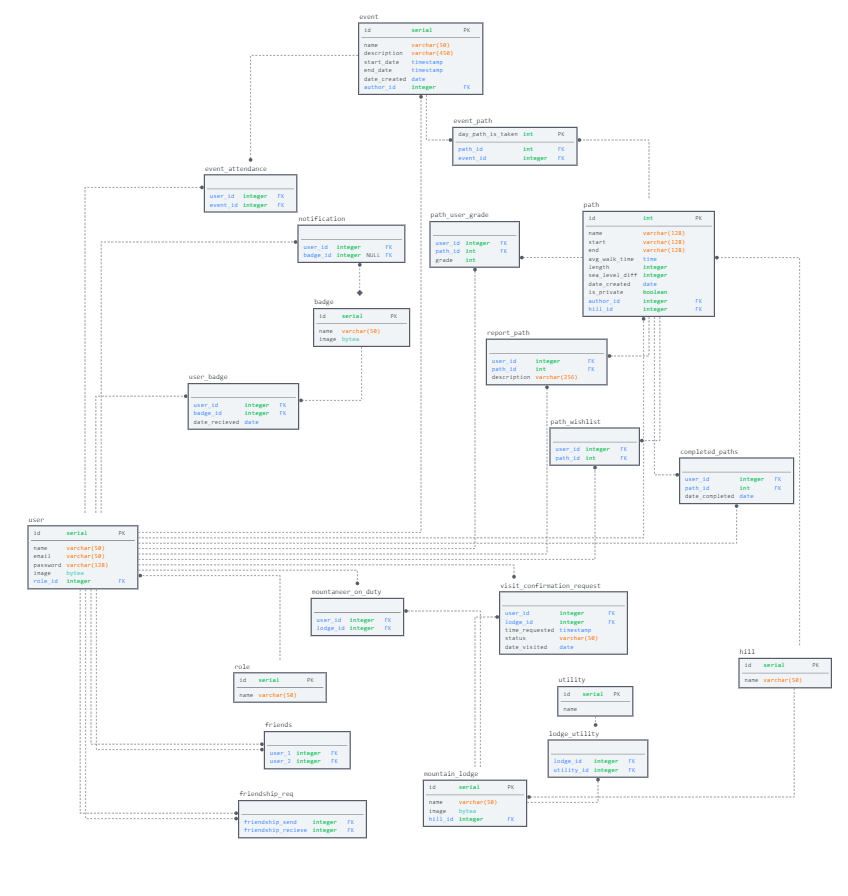
\includegraphics[width=\linewidth]{slike/database.png}
			
			\eject
			
			
		\section{Dijagram razreda}
		
			\textit{Potrebno je priložiti dijagram razreda s pripadajućim opisom. Zbog preglednosti je moguće dijagram razlomiti na više njih, ali moraju biti grupirani prema sličnim razinama apstrakcije i srodnim funkcionalnostima.}\\
			
			\textbf{\textit{dio 1. revizije}}\\
			
			\textit{Prilikom prve predaje projekta, potrebno je priložiti potpuno razrađen dijagram razreda vezan uz \textbf{generičku funkcionalnost} sustava. Ostale funkcionalnosti trebaju biti idejno razrađene u dijagramu sa sljedećim komponentama: nazivi razreda, nazivi metoda i vrste pristupa metodama (npr. javni, zaštićeni), nazivi atributa razreda, veze i odnosi između razreda.}\\
			
			\textbf{\textit{dio 2. revizije}}\\			
			
			\textit{Prilikom druge predaje projekta dijagram razreda i opisi moraju odgovarati stvarnom stanju implementacije}
			
			
			
			\eject
		
		\section{Dijagram stanja}
			
			
			\textbf{\textit{dio 2. revizije}}\\
			
			\textit{Potrebno je priložiti dijagram stanja i opisati ga. Dovoljan je jedan dijagram stanja koji prikazuje \textbf{značajan dio funkcionalnosti} sustava. Na primjer, stanja korisničkog sučelja i tijek korištenja neke ključne funkcionalnosti jesu značajan dio sustava, a registracija i prijava nisu. }
			
			
			\eject 
		
		\section{Dijagram aktivnosti}
			
			\textbf{\textit{dio 2. revizije}}\\
			
			 \textit{Potrebno je priložiti dijagram aktivnosti s pripadajućim opisom. Dijagram aktivnosti treba prikazivati značajan dio sustava.}
			
			\eject
		\section{Dijagram komponenti}
		
			\textbf{\textit{dio 2. revizije}}\\
		
			 \textit{Potrebno je priložiti dijagram komponenti s pripadajućim opisom. Dijagram komponenti treba prikazivati strukturu cijele aplikacije.}